\documentclass{article} % For LaTeX2e
\usepackage{nips14submit_e,times}
\usepackage{amsmath}
\usepackage{amsthm}
\usepackage{amssymb}
\usepackage{mathtools}
\usepackage{hyperref}
\usepackage{url}
\usepackage{algorithm}
\usepackage[noend]{algpseudocode}
%\documentstyle[nips14submit_09,times,art10]{article} % For LaTeX 2.09

\usepackage{mathrsfs}
\usepackage{graphicx}
\usepackage{caption}
\usepackage{subcaption}

\def\eQb#1\eQe{\begin{eqnarray*}#1\end{eqnarray*}}
\def\eQnb#1\eQne{\begin{eqnarray}#1\end{eqnarray}}
\providecommand{\e}[1]{\ensuremath{\times 10^{#1}}}
\providecommand{\pb}[0]{\pagebreak}


\def\Qb#1\Qe{\begin{question}#1\end{question}}
\def\Sb#1\Se{\begin{solution}#1\end{solution}}

\newenvironment{claim}[1]{\par\noindent\underline{Claim:}\space#1}{}
\newtheoremstyle{quest}{\topsep}{\topsep}{}{}{\bfseries}{}{ }{\thmname{#1}\thmnote{ #3}.}
\theoremstyle{quest}
\newtheorem*{definition}{Definition}
\newtheorem*{theorem}{Theorem}
\newtheorem*{lemma}{Lemma}
\newtheorem*{question}{Question}
\newtheorem*{preposition}{Preposition}
\newtheorem*{exercise}{Exercise}
\newtheorem*{challengeproblem}{Challenge Problem}
\newtheorem*{solution}{Solution}
\newtheorem*{remark}{Remark}
\usepackage{verbatimbox}
\usepackage{listings}

\title{Real Variables: \\
Problem Set X}


\author{
Youngduck Choi \\
Courant Institute of Mathematical Sciences \\
New York University \\
\texttt{yc1104@nyu.edu} \\
}


% The \author macro works with any number of authors. There are two commands
% used to separate the names and addresses of multiple authors: \And and \AND.
%
% Using \And between authors leaves it to \LaTeX{} to determine where to break
% the lines. Using \AND forces a linebreak at that point. So, if \LaTeX{}
% puts 3 of 4 authors names on the first line, and the last on the second
% line, try using \AND instead of \And before the third author name.

\newcommand{\fix}{\marginpar{FIX}}
\newcommand{\new}{\marginpar{NEW}}

\nipsfinalcopy % Uncomment for camera-ready version

\begin{document}


\maketitle

\begin{abstract}
This work contains solutions to the problem set 
X of Real Variables 2015 at NYU.
\end{abstract}

\section{Solutions}

\begin{question}[1. Royden 13-41]
\hfill
\begin{figure}[h!]
  \centering
    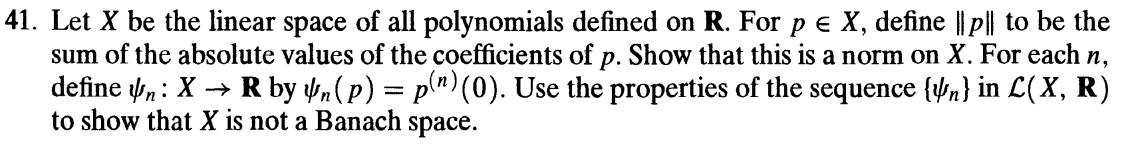
\includegraphics[width=1\textwidth]{13-41.png}
\end{figure}
\end{question}
\begin{solution} We first show that $\lVert \> \rVert:X \to \mathbb{R}$
given is a norm on $X$. First of all, let $p = 0$. Then, $\lVert p \rVert
= 0$. Now, let $p = \sum_{i=0}^{n} b_i x^i$, and 
assume that $\lVert p \rVert = 0$. It follows that $\sum_{i=0}^{n} |b_i| 
= 0$. As $|b_i| \geq 0$ for all $i$, we have that $b_i = 0$ for all $i$. 
Hence, $p = 0$. For proving the triangle inequality,
let $p_1 = \sum_{i=0}^{n_1} b_i x^i$ and $p_2 = \sum_{i=0}^{n_2} c_i x^i$. 
Without the loss of generality, we assume that $n_1 \geq n_2$, and 
define $n = n_1$, $p_1 = \sum_{i=0}^{n} b_i x^i$ 
and $p_2 = \sum_{i=0}^{n} c_i x^i$, with $c_i = 0$ for $i > n_2$.  
By the triangle inequality of reals, it follows that
\eQb
\lVert p_1 + p_2 \rVert &=& \lVert \sum_{i=0}^{n} (b_i + a_i) x^i \rVert \\
&=& \sum_{i=0}^{n} |b_i + a_i| \\
&\leq& \sum_{i=0}^{n} |b_i| + |a_i| \\
&=& \sum_{i=0}^{n} |b_i| + \sum_{i=0}^{n} |c_i | =
\lVert p_1 \rVert + \lVert p_2 \rVert.
\eQe 
Now, let $p = \sum_{i=0}^{n} b_i x^i$, and $\alpha \in \mathbb{R}$. 
It follows that 
\eQb
\lVert \alpha p \rVert &=& \lVert \alpha \sum_{i=0}^{n} b_i x^i \rVert \\
&=& \lVert \sum_{i=0}^{n} \alpha b_i x^i \rVert \\
&=& \sum_{i=0}^{n} |\alpha b_i | \\
&=& |\alpha| \sum_{i=0}^{n} |b_i| = |\alpha| \lVert p \rVert . 
\eQe 
Hence, we have shown that $\lVert \> \rVert$ given is a norm.

\smallskip

Now, we first show that each operator $\psi_n$ is bounded, thus continuous.
Observe that we can represent an arbitrary polynomial $p$ uniquely as ,
for some $k$, 
$p = \sum_{i=0}^{\infty} c_i x^i$, where $c_i = 0$ for $i \geq k$. 
Fix $\psi_n$.
Observe that for any $p$, we have $|c_n| \leq \lVert p \rVert$. 
It follows that 
\eQb
|\psi_n(p) | &=& |n! \cdot c_n | \\
&=& |n!| |c_n| \\
&\leq& |n!| \lVert p \rVert \\ 
\eQe 
Hence, $\psi_n$ is bounded, thus continuous for any $n$. Note that 
by taking $p = x^n$, we obtain $n! \leq M$ for any bound $M$ for $\psi_n$.
Hence, it follows that $\lVert \psi_n \rVert = n!$.
Again, for any polynomial $p$, observe that $\psi_n(p) = 0$ for $n > k$,
where $k$ denotes the degree of the polynomial $p$. Consequently, we 
have 
\eQb
\lim_{n \to \infty} \psi_n(p) &=& 0,
\eQe
for any $p$. Therefore, if $X$ is Banach, the conditions of 
the Banach-Saks-Steinhaus theorem is satisfied. However, as $\lVert \psi_n
\rVert = n!$, $\{ \psi_n\}$ cannot be uniformly bounded. This is a 
contradiction. $X$ is not Banach.

 
\end{solution}

\newpage

\begin{question}[2. Royden 14-18]
\hfill
\begin{figure}[h!]
  \centering
    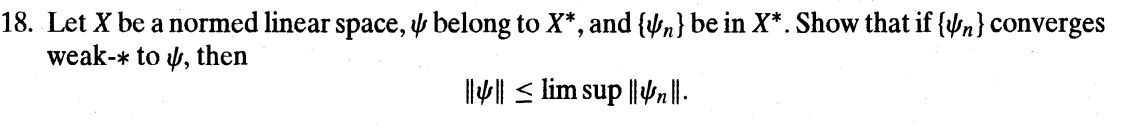
\includegraphics[width=1\textwidth]{14-18.png}
\end{figure}
\end{question}
\begin{solution}
As $\{ \psi_n \}$ is weak-* convergent to $\psi$, we have 
\eQb
\psi_n(x) &\to& \psi(x),
\eQe
for all $x \in X$. Let $x \in X$.
As $| \cdot |$ is continuous on $\mathbb{R}$,
it follows that
\eQb
\lim_{n \to \infty} |\psi_n(x)| &=& |\psi(x)|. 
\eQe 
As $|\psi_n(x) | \leq ||\psi_n || \cdot ||x||$, 
\eQb
|\psi(x)| &=& \lim_{n \to \infty} |\psi_n(x)| \\
&=& \limsup_{n \to \infty} |\psi_n(x)| \\ 
&\leq&\limsup_{n \to \infty} ||\psi_n || \cdot ||x|| \\
&=& ||x|| \limsup_{n \to \infty} ||\psi_n||.
\eQe
Since $x \in X$ was arbitrary,  it follows that
\eQb
||\psi|| &\leq& \limsup_{n \to \infty} ||\psi_n||, 
\eQe
as desired. \hfill $\qed$
\end{solution}

\newpage

\begin{question}[3. Royden 14-23]
\hfill
\begin{figure}[h!]
  \centering
    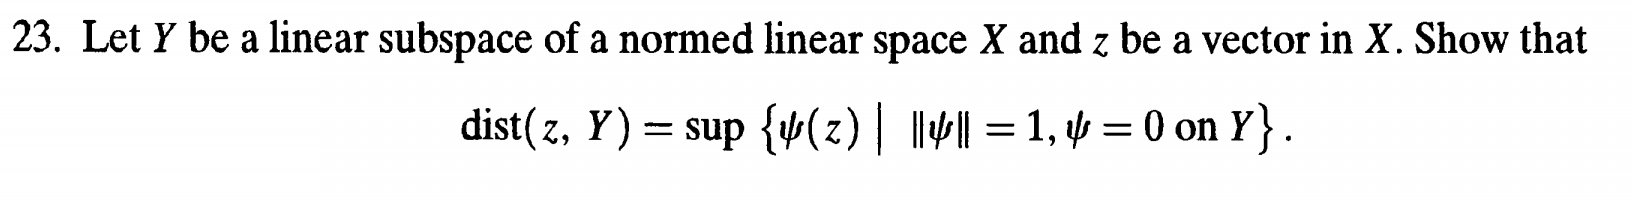
\includegraphics[width=1\textwidth]{14-23.png}
\end{figure}
\end{question}
\begin{solution}
I believe there is an error in this problem. 
\end{solution}

\newpage

\begin{question}[4. Royden 15-12]
\hfill
\begin{figure}[h!]
  \centering
    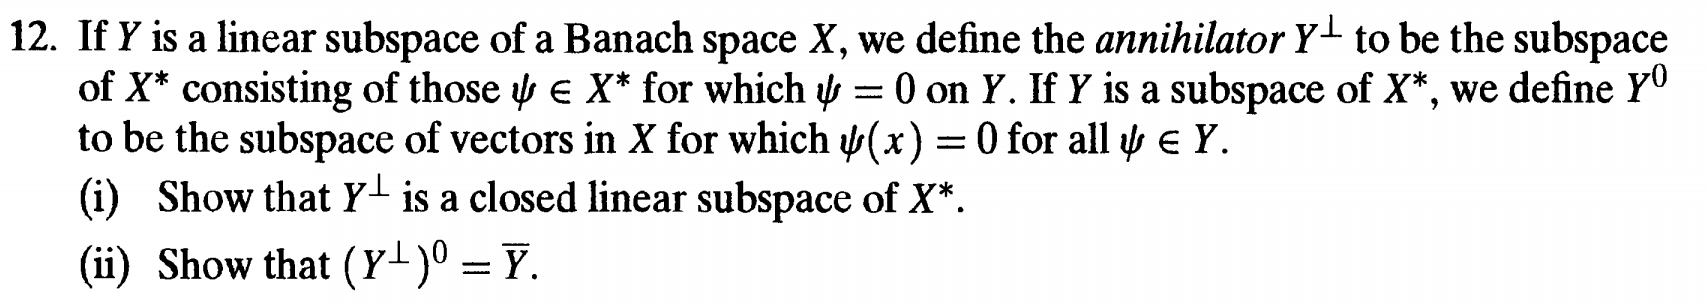
\includegraphics[width=1\textwidth]{15-12.png}
\end{figure}
\end{question}
\begin{solution}
\textbf{(i)} For $x \in X$, let $Y_{x}^{\perp}$ be defined by
\eQb
Y_{x}^{\perp} &=& \{ \psi \in X^* \> | \> \psi(x) = 0 \}.
\eQe
As $\psi \in X^*$, $\psi$ is continuous, hence $Y_{x}^{\perp}$ is
closed. Observe that
\eQb
Y^{\perp} &=& \bigcap_{x \in Y}  Y_{x}^{\perp}.
\eQe
Each $Y_{x}^{\perp}$ is closed, since a limit function of continuous functions
with respect to the operator norm, will preserve the property that
$0$ will be achieved at $x$.
Since an arbitrary intersection of closed sets is closed, we have that
$Y^{\perp}$ is closed linear subspace of $X^*$.

\bigskip

\textbf{(ii)} First, we show that $(Y^{\perp})^0$ is closed. Observe
that 
\eQb
(Y^{\perp})^{0} &=& \bigcap_{\psi \in Y^{\perp}} \{ x \in X \> | \>
\psi(x) = 0 \} \\
&=& \bigcap_{\psi \in Y{^\perp}} \psi^{-1}(0).
\eQe
As $\psi^{-1}(0)$ is a pre-image of a single point, which is closed in 
a metric space, of a continuous function, and intersection of closed sets
is closed, we have that $(Y^{\perp})^{0}$ is closed. By definition of 
$Y^{\perp}$, it follows that $Y \subseteq (Y^{\perp})^0$, and as 
$(Y^{\perp})^0$ is closed, we obtain $\overline{Y} \subseteq (Y^{\perp})^0$.
Now, we show that $(Y^{\perp})^0 \subseteq \overline{Y}$ holds. It suffices
to show that $X\setminus \overline{Y} \subseteq X \setminus 
(Y^{\perp})^0$ holds. 
Let $x \in X\setminus \overline{Y}$. Then, we know that there exists 
$\psi \in X^*$ such that $\psi(x) \neq 0$ and $\ker(\psi)$ contains $Y$.
Hence, $x \notin (Y^{\perp})^{0}$. Therefore, we have shown that
$Y = (Y^{\perp})^0$ as desired. \hfill $\qed$
 
\end{solution}
\end{document}
